
\begin{frame}{Feature Template: One-Hot Encoding}
\begin{definition}
A \textbf{one-hot encoding }is a set of features (e.g. a feature template)
that always has \textbf{exactly one} non-zero value. 

\pause{}
\end{definition}

\begin{center}
\includegraphics[height=0.5\textheight]{../Figures/features/lastCharacter\lyxdot oneHot} 
\par\end{center}
\let\thefootnote\relax\footnotetext{\tiny{From Percy Liang's "Lecture 3" slides from Stanford's CS221, Autumn 2014. }}
\end{frame}


\begin{frame}{Feature Template: Count-based}
\begin{itemize}
	\item Imagine you're working on an internet scale problem (ex:  click-through rate prediction).
	\item What might be a problem with one-hot encoding raw features (domains, etc.) in problems at this scale?
\end{itemize}
\end{frame}


\begin{frame}
\begin{center}
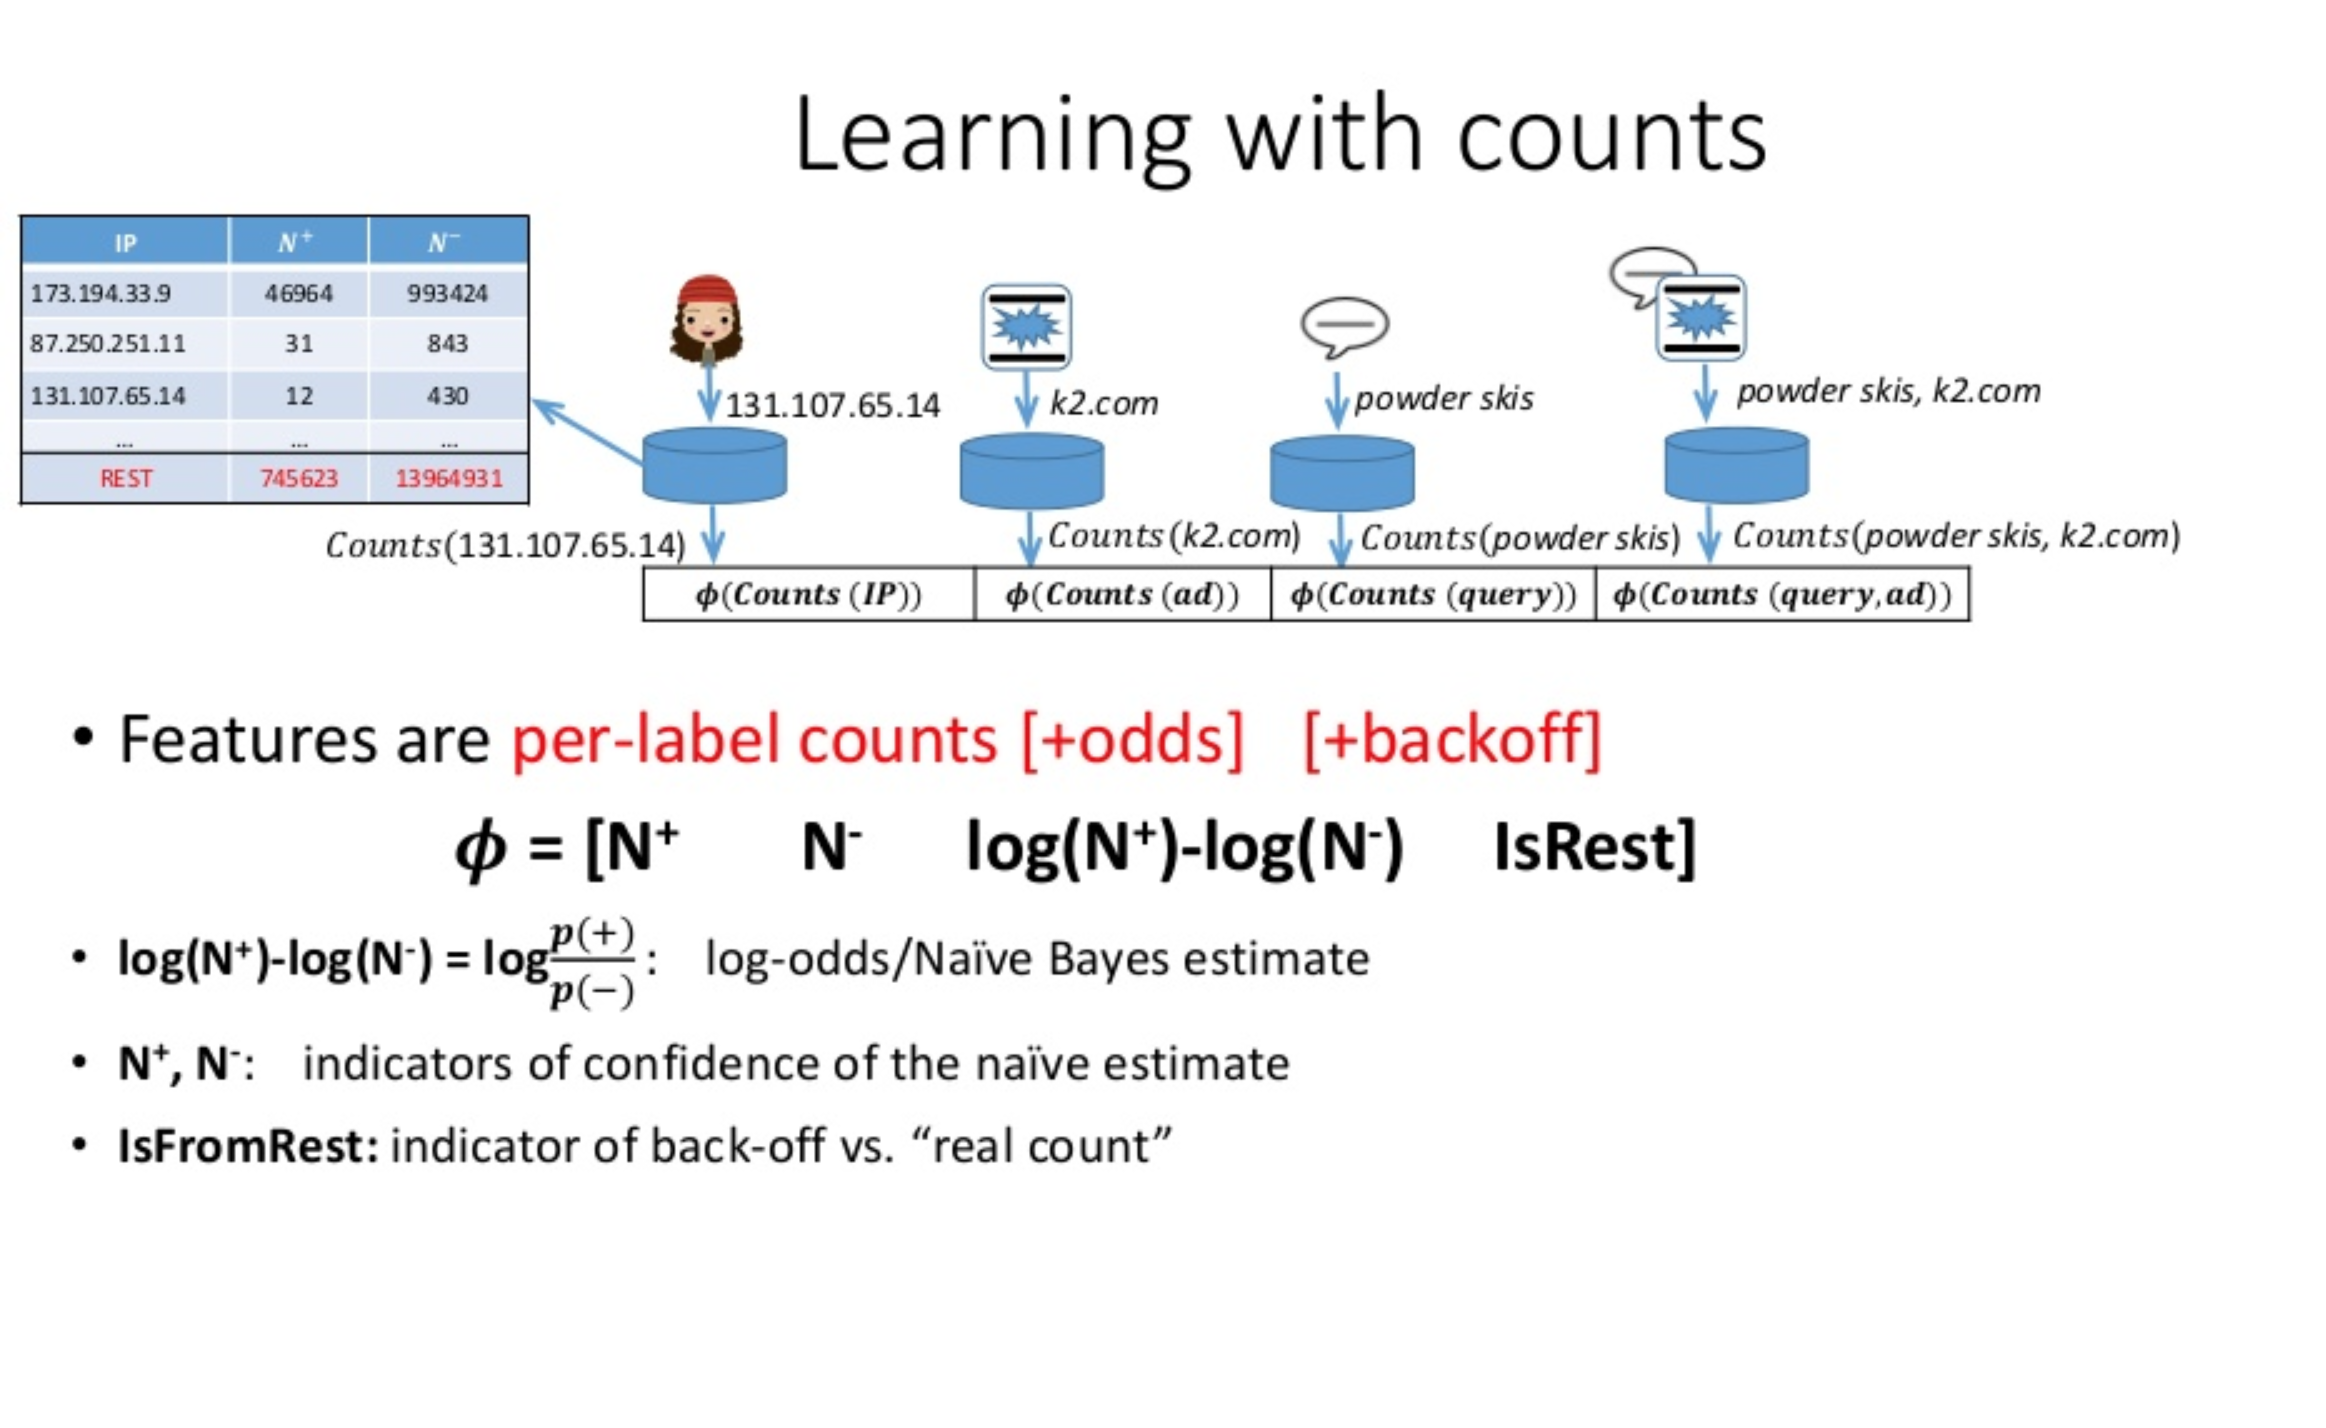
\includegraphics[height=0.9\textheight]{../Figures/learn_with_counts.png} 
\par\end{center}
\let\thefootnote\relax\footnotetext{\tiny{From Misha Bilenko/Microsoft Azure ML's ``Many Shades of Scale: Big Learning Beyond Big Data"}}
\end{frame}
